\chapter{Shared Resources}
So far we have assumed that all tasks can run and compete for a processor indipendently (i.e. do not interact with one another).

However there are several occasions in which this assumption can simply not be made: the most evident is when two tasks have to share information and/or exchange variables, another scenario can happen when two or more tasks have to compete for shared resources.

So in this chapter we will look into this aspect and in particular we will start talking about the notion of atomicity.

\section{The notion of atomicity}
\side{Atomocity}: an hardware instruction is atomic if it cannot be ``interleaved'' with other instructions. \\
In other terms, even if there are instructions/activities/tasks with higher priority, an atomic instruction will carry on its execution without interruption until it has finished.

Moreover:
\begin{itemize}
\item atomic operations are \side{always sequentialized}
\item atomic operations \side{cannot be interrupted}
\begin{itemize}
\item they are safe operations
\item e.g., transferring one word from memory to register or viceversa. It cannot be allowed that someone access/modify the word while it is transferring into a register, hence the task/instruction responsible for moving into the register the word has to be an atomic instruction.
\end{itemize}
\item non atomic operations can be interrupted
\begin{itemize}
\item they are not ``safe'' operations
\item non elementary operations are not atomic
\end{itemize}
\end{itemize}

Usually, you prefer to have, whenever possible, non atomic operations because they are the ones that allow you to exploit in full the possibility to schedule the processor to activities having an higher priority.

\subsection{Non atomic operations}
Consider a simple, increment operation:
\[x=x+1\]
in assembler, this expression would probably take the form:
\begin{lstlisting}[language={[x86masm]Assembler}]
LD   R0, x
INC  R0
ST   x, R0
\end{lstlisting}
where the variable $x$ is loaded into a register $R0$, the register will then be incremented and the result will be stored into $x$.

\subsubsection{Interrupt on non-atomic operations}

A simple operation like incrementing a memory variable, may be composed by three machine instructions.

If the same operation is done inside an \side{interrupt handler} (routing executed in response to an interrupt), an inconsistency can arise:
\begin{figure}[!h]
\centering
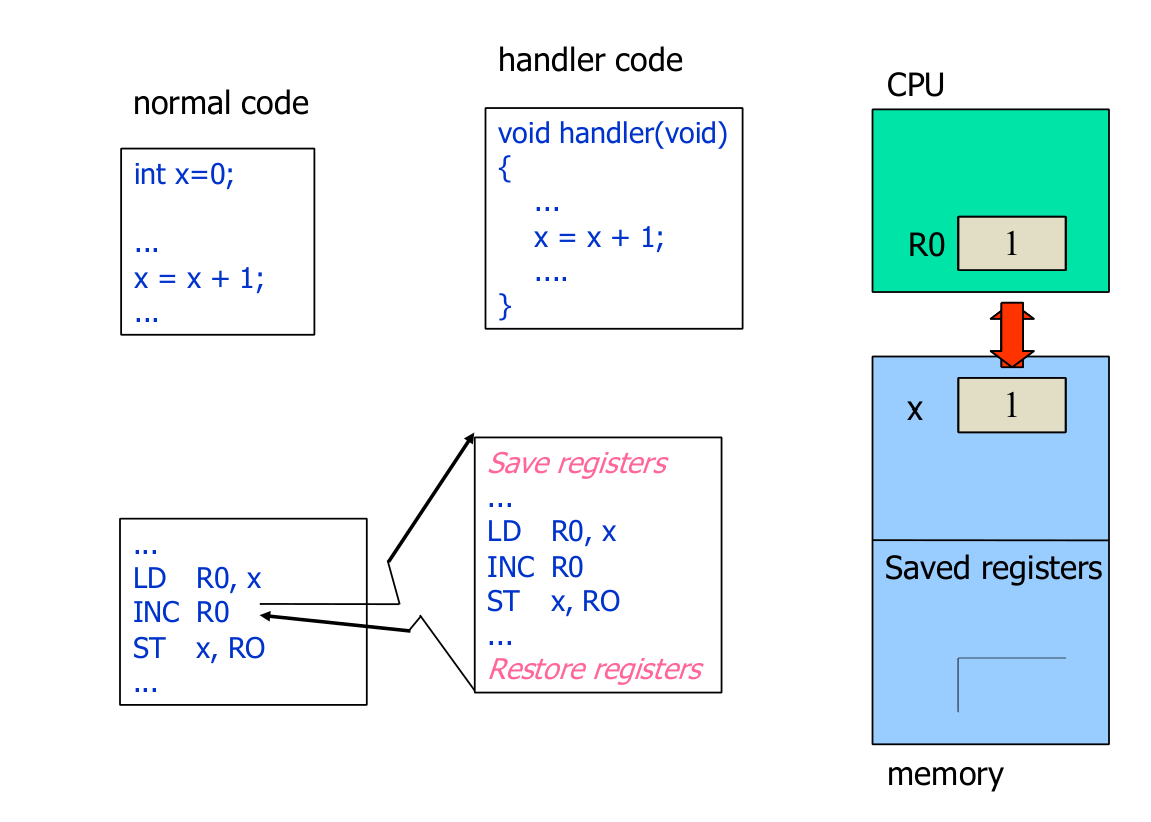
\includegraphics[width=.7\textwidth]{image06}
\end{figure}
The normal code starts to execute:
\begin{enumerate}
\item The value of $x$ is set to 0 in memory
\item The value of $x$ is copied into the register $R0$
\item Before the increments something happens that triggers the execution of the interrupt handler
\item The interrupt handler creates a copy of all the registers (that contains the value of $x$), and then it executes its incrementation of $R0$.
\item The interrupt handles finishes and all the saved registered values are loaded back in/restored.

Hence the normal code assumes that $x$ is zero (which is the value of the register before the interrupt) and increments it by one and stores it into $x$.
\item Eventually, $x$ will be equal to 1. From a logical point of view two increments should have taken place, but in fact one of them was not successfully completed, because during the execution fo the increment I was allowed to be interrupted.
\end{enumerate}
The issue with this scenario is that it does not always happen like this: sometimes the normal code is able to complete before the interrupt is fired.
Under this circumstance, we would see that the variable $x$ is incremented both times instead of one.

This condition is known as \side{Critical race}, because you can have multiple execution of the code that interleave their operations in slightly different way and obtain different results. And in fact, this is one of the nastiest problem in computer science and computer engineering, because sometimes the problem does not materialize for years.

\subsubsection{Task concurrency in non-atomic operations}
The reason why this problem is not easy to debug and notice is that we cannot make any assumption in advance about the relative speed of the processes, hence, we do not know the order of execution of the hardware instructions.\\
Moreover, you cannot make any assumption on when certain events are triggered, because you can have jitter in the generation of the interrupt. 

Recall the example of incrementing variable $x$. 
\begin{itemize}
\item Incrementing $x$ is not an atomic operation, that instead should be.
\item atomic behaviour can be obtained using interrupt disabling or special atomic instructions. A simple solution then is disabling the interrupt before the execution of the normal code and resuming them after the execution of the code has ended.
\end{itemize}

Clearly, the same bad interleaving problem can happen in case of concurrent task as displayed in figure \ref{fig:sec4ex1}:
\begin{enumerate}
\item Consider two concurrent tasks, such that the priority of B is higher than A, and a shared memory approach
\item Normally when task B starts it interrupts task A, It could happen that task B starts right after task A has taken its snapshot of the variable $x$
\item What you come up with is exactly the same problem as before: sometimes the variable will be 2 and sometimes it will be 1.
\end{enumerate}

\missingfigure{example 1}

The same situation can happen in more convoluted problems:
\begin{enumerate}
\item Consider a struct with two fields ($a$, $b$), with some functions that operates on the data structure.
\item And assume that we have two tasks A and B, which call respectively, two different methods.
\item If A start executes and increments $a$ and gets interrupted before incrementing $b$, resulting in a non consistent state
\end{enumerate}
\missingfigure{example 2}

\section{Critical sections}
At this point, we can provide the reader with some definitions that will be important for the follow up of our discussion.
\subsection{Definitions}
\begin{itemize}
\item the \side{shared object} where the conflict may happend in a \side{resource}.

A resource shared by two or more threads, shared by a thread and an interrupt handler or etc...
\item the \side{parts of the code} where the problem may happen are called \side{critical sections}.

A critical section is a sequence of operations that cannot be interleaved with other operations on the same resource.
\item Two critical sections on the same resource must be properly sequentialized.
\item we say that two critical sections on the same resource must execute in \side{Mutual exclusion}. Two critical sections cannot be executed at the same time, but one needs to stand by when the other executes.
\item There are three ways to obtain mutual exclusion:
\begin{enumerate}
\item implementing the \side{critical section as an atomic operation} (i.e. disabling interrupts before executing the operation, and restoring interrupts at the end). This approach is really tough and extreme to implement because if one disables the interrupts, the I/O system of the machine is no longer allowed to work properly.
\item \side{disabling the preemption (system-wide)}, for instance by raising the priority of the critical section/of the task to the maximum in the system and restoring back the priority at the end. However, this approach has some drawbacks because all the tasks will suffer from this suspension fo the preemption even though they do not use the shared resources.
\item \side{selectively disabling the preemption} (using semaphores and mutual exclusion). I.e. preemption will be disabled only for the task that operates on the shared resource.
\end{enumerate}
\end{itemize}

\subsubsection{Atomic operations}
If we implement a critical section as an atomic operations, implies that the interrupts are disabled suring the execution of such critical section. In order to do so, Assembler language provides the \texttt{CLI} instruction and restore the interrupts right at the end of the execution via \texttt{STI}.

Problems:
\begin{itemize}
\item If the critical section is long, no interrupt can arrive during the critical section.

e.g. consider a timer interrupt that arrives every 1 ms. If a critical section lasts for more than 1 ms, a timer interrupt could be lost.
\item Concurrency is disabled during the critical section: we must avoid conlict on the resource, not disabling interrupts!
\end{itemize}

\subsubsection{Disabling preemption system-wide}
Instead of disabling interrupts, it is ar more safer to disable preemption. It is, in fact, possible to disable preemption for a limited interval of time.

Consider a task that is normally non preemptive (i.e. cannot be interrupted by anyone). Such task can execute the critical section without interruption, then the function schedule is called signaling that some other task having a higher priority can take over.

\begin{lstlisting}[language=C++]
TASK(A) // <- all the task is non preemptive
{
...
<critical section> 	// no context switch may happen during the critical section
Schedule();		// context switch, allows execution of higher priority tasks
<critical section>	// the function schedule returns: TASK(A) has the higher priority task
...
}
\end{lstlisting}

This is what happens in OSEK (a kind of RTOS, widely used in cars), that use ono-preemptive tasks together with the \texttt{Schedule()} primitive.

Problems: if a high priority critical thread needs to execute, it cannot make preemption and it is delayed, even if the high priority task does not access the resource.

\subsubsection{Selectively disabling preemption}
The best way to implement mutual exclusion is by selectively disable preemption.

There exist some general mechanisms to implement mutual exclusion only between the processes that use a resource: OSEK, for instance, uses the GetResource/ReleaseResource primitive (in POSIX there is mutex\_lock and mutex\_unlock):

\begin{minipage}{0.475\textwidth}
\centering
\begin{lstlisting}[language=C++]
TASK(A)
{
...
GetResource(r);
<critical section>
ReleaseResource(r);
...
}
\end{lstlisting}
\end{minipage}
\hfill
\begin{minipage}{0.475\textwidth}
\centering
\begin{lstlisting}[language=C++]
TASK(B)
{
...
GetResource(r);
<critical section>
ReleaseResource(r);
...
}
\end{lstlisting}
\end{minipage}

\subsection{Schedulability and critical sections}

Up to now, we have considered \side{independent tasks}. However tasks do interact between each other: they use shared data, non preemptable resources, etc...

The big issue is that when one disables preemption (even selectively) the priority mechanism is no longer enforced: a task with lower priority for the lenght of the critical section will execute instead of an higher priority task (it operates as if it had the highest priority).



This issue is commonly known as \side{priority inversion}: period in which a high priority task is prevented from executing by a low priority task. If priority inversion is not correctly manages it may result in a violation of timing constraits.


\section{Interacting Tasks}

Until now, only independent tasks:
\begin{itemize}
\item A job never block or suspends
\item A task only block on job termination
\end{itemize}
In real world, jobs migh bloc for various reasons:
\begin{itemize}
\item Tasks exchange data through shared memory (mutual exclusion)
\item A task might need to synchronize with other tasks while waiting for some data
\item A job might need a hardware resource which is currently not available
\end{itemize}

Example: Consider a contorl application composed by three periodic tasks:
\begin{itemize}
\item $\tau_1$ reads the data from the sensors and applies a filter. The results are stored in memory
\item $\tau_2$ reads the filtered data and computes some control law (updating the state and the outputs); both the state and the outputs are stored in memory
\item $\tau_3$ reads the outputs and writes on an actuator
\end{itemize}

All o the three tasks access data in shared memory, hence when they execute concurrently, if we do not schedule/manage the resources properly it may happen that some data structure (in the information exchange) could be corrupted/inconsistent (a task can read a piece of the structure before the task responsible to providing it has finished modifying it).

\subsection{Task Intraction Paradigms}

The possible ways of managing interactions between tasks are:
\begin{itemize}
\item \side{Private Resources} (Client/Server paradigm)
\item \side{Shared Resources}
\end{itemize}

\subsubsection{Private Resources}

The resources are privatly handlesd by a task. Hence a \side{Resource Manager} (aka server task) per resource is instantiated.
This method is based on processes, i.e. they have their own address space (direct access to the resource).

In case some other tasks would like to access and use a resource, it would send a message/request to the relative manager of the resource via Inter-Process Communication .

This is the same mechanism that we use when accessing the web.

\subsubsection{Shared Resources}
Another approach is to consider shared resources: resources are no longer privately owned by any task, but it is possible for all the tasks to have access to the resources.\\
This is a shared memory model, as such it is based on multithreaded programming (multiple thread of execution, but address space is the same).\\
This interaction happens via mutexes, semaphores, condition variables, ...


\subsection{Resources and Critical sections}

If you look into both approaches, you will quickly realise that at some point there will be a problem of concurrency: especially in reading and writing to its resources.\\
You can have the impression that when using a multiprocess based on the model of private resources you have evaded the problem, but in reality not.\\
For sake of simplicity we will analyze the problem for the case of shared resources:
\begin{itemize}
\item We will use mutexes (specifically devoted to the issue of implementing mutual exclusion) and not semaphores (can be used a mutually exclusive region, but also for general purpose synchronization).
\item Extensions to IPC based communication are possible.
\end{itemize}

On the frame of reference of the interacting tasks, we can redefine it as a schedulable entity or active entity that can perform operatinos on private or shared data.

Focusing on shared data, we need to model the mechanism that protects such shared data: as a consequence, the shared data that get protected by mutual exclusive objects (aka mutexes) is called protected object.

In other terms, \side{Protected Objects}:
\begin{itemize}
\item Encapsulate shared information (\side{Resources})
\item \side{Passive Objects} (data) shared between different tasks
\item Operations on protected objects are mutually exclusive (i.e. protected)
\end{itemize}

In order to protect the object:
\begin{itemize}
\item A mutex variable gets locked at the beginning, so that a task becomes the owner of the associated resource
\item At this point when the task has locked the resource and before it releases the lock, the task effectively owns the resource
\end{itemize}

\subsection{Shared Resources}

A \side{Shared Resource} $S_i$
\begin{itemize}
\item can be used by multiple tasks
\item is protected by a mutex (mutual exclusion semaphone)
\item has a 1 to 1 relationship between resources and mutexes.

Convention: $S_i$ can be used to indicate either the resource or the mutex
\end{itemize}
In order to make real time scheduling analysis with this concept in ming we need to extend our system model according to this definition; now the system is not limited to a set of tasks...

\subsubsection{System Model}
A system/Application can be modeled by:
\begin{itemize}
\item A set $\mathcal{T}$ of $N$ periodic (or sporadic) tasks:
\[\mathcal{T} = \{\tau_i : 1\le i\le N\}\]
\item A set $\mathcal{S}$ of $M$ shared resources:
\[\mathcal{S}=\{S_i : 1 \le i \le M\}\]
\item Task $\tau_i$ uses resource $S_j$ if it accesses the resource (in a critical section)
\item The $k$-th critical section of task $\tau_i$, that uses the resource $S_j$ will be called:
\[cs_{i,j}^k\]
\item The length of the longest critical section of $\tau_i$ on $S_j$ will be $\xi_{i,j}$
\end{itemize}

\subsubsection{Blocking Time}
The consequences of using this method and model when it comes to evaluating the timing behavior of the task.
We will need to introduce the definition of \side{Blocking time}, i.e. the time that a task has to wait for a resource to be released.

Formally:
\begin{itemize}
\item When task $\tau_i$ tries to access a resource $S$ already held from task $\tau_j$, $\tau_i$ blocks
\item Blocking time: time between the instant when $\tau_i$ tries to access $S$ (and blocks) and the instant when $\tau_j$ releases $S$ (and $\tau_i$ unblocks)
\end{itemize}

Note that this is needed for implementing mutual exclusion and cannot be avoided. Notice that when we talk about blocking time we refer to the time a task has to wait when somebody having a priority lower than it owns a resource (not higher).\\
Clearly if this blocking time becomes too large, then the very mechanism of scheduling priorities that allowed me to guarantee the timely execution of the task is disrupted.

Blocking times can be particularly bad in priority scheduling if a high priority task wants to access a resource that is held by a lower priority task: a lowe priority task executes, while a high priority one is blocked; schedulability guarantees can be compromised.


We need to find means to account for the blocking time: in fact, if this blocking time was limited or bounded than we can account for it in the WCET of the task, but this is possile only if this blocking times are deterministic and not too large.

